\documentclass[11pt,a4paper]{article}

\usepackage[margin=1in, paperwidth=8.3in, paperheight=11.7in]{geometry}
\usepackage{amsmath,amsfonts,fancyhdr,bbm,tikz}
\usetikzlibrary{arrows,automata}
\usepackage[section,nohyphen]{DomH}
\headertitle{Stochastic Optimisation - Problem Sheet 2}

\begin{document}

% \questionsfalse
% \answersfalse

\title{Stochastic Optimisation - Problem Sheet 2}
\author{Dom Hutchinson}
\date{\today}
\maketitle

\begin{question}{1.}
  Consider a bandit with two independent arms, where the rewards from arm $i$ are i.i.d. with a $\text{Normal}(i, i)$ distribution, $i\in\{1,2\}$. In other words, rewards from arm $i$ are normally distributed with mean $i$ and variance $i$, so that the second arm has the larger mean reward.
  \par Fix a time horizon $T$, and consider the heuristic which first plays each arm exactly $n$ times, and subsequently plays the arm with the higher sample mean reward.
\end{question}

\begin{question}{1. (a)}
  Let $\hat\mu_{1,n}$ and $\hat\mu_{2,n}$ denote the samples means of the first $n$ plays of arm 1 and 2 respectively. Using the answer to \texttt{Problem Sheet 1 Q6 (b)}, obtain an upper bound on
  \[ \prob(\hat\mu_{1,n}\geq\hat\mu_{2,n}) \]
\end{question}

\begin{answer}{1. (a)}
  Let random variables $X_i(t)\sin\text{Normal}(i,i)$ for $i\in\{1,2\}$ model the reward received from arm $i$ at time $t$ and $\hat\mu_{i,n}$ denote the sample mean from the first $n$ times arm $i$ is played.
  \par Define random variable $X(t):=X_1(t)-X_2(t)$ which has distribution $\text{Normal}(1-2,1+2)=\text{Normal(-1,3)}$ and $\hat\mu_n:=\frac1n\sum_{i=1}^nX(t)=\hat\mu_{1,n}-\hat\mu_{2,n}$. Thus
  \[\begin{array}{rcl}
    \prob(\hat\mu_{1,n}\geq\hat\mu_{2,n})&=&\prob(\hat\mu_{1,n}-\hat\mu_{2,n}\geq0)\\
    &=&\prob(\hat\mu_n\geq0)\\
    &=&\prob\left(\frac1n\sum_{i=1}^nX_i\geq0\right)\\
    &=&\prob\left(\sum_{i=1}^nX_i\geq0\right)
  \end{array}\]
  \texttt{Problem Sheet 1 Q6 b)} states that for IID random variables $X_1,X_2,\dots$ with distribution $\text{Normal}(\mu,\sigma^2)$ and for $\gamma>\mu$, the following bound exists.
  \[ \prob\left(\sum_{i=1}^nX_i\geq n\gamma\right)\leq\exp\left(-n\frac{(\gamma-\mu)^2}{2\sigma^2}\right) \]
  By defining $\gamma=0$ and noting that $\gamma>\mu=-1$ we can apply this result to the inequality above.
  \[\begin{array}{rrcl}
    &\prob\left(\sum_{i=1}^nX_i\geq0\right)&\leq&\exp\left(-n\frac{(0-(-1))^2}{2\cdot3}\right)\\
    &&=&\exp\left(-\frac{n}6\right)\\
    \implies&\prob(\hat\mu_{1,n}\geq\hat\mu_{2,n})&\leq&\exp\left(-\frac{n}6\right)
  \end{array}\]
\end{answer}

\begin{question}{1. (b)}
  Using the answer to the last part, find an upper bound on the regret, $\R(T)$, of this heuristic. Optimize this upper bound over $n$, treating $n$ as if it were a real number, and approximating quantities like $T-n$ by $T$, on the assumption that $n$ is much smaller than $T$.
\end{question}

\begin{answer}{1. (b)}
  The algorithm here can be considered to have two stages: learning; and post-learning. During the learning phase we are guaranteed to play the sub-optimal arm $n$ times, but we play the same arm throughout the post-learning phase and thus regret only increases if the wrong arm is made (ie if $\hat\mu_{1,n}\geq\hat\mu_{2,n}$).\\
  Note that the post-learning phase consists of $(T-2n)$ rounds and the loss incurred from playing the sub-optimal arm is $2-1=1$.
  \[\begin{array}{rcl}
    \R_T&=&\underbrace{1\cdot n}_\text{learning}+\underbrace{1\cdot(T-2n)\prob(\hat\mu_{1,n}\geq\hat\mu_{2,n})}_\text{wrong choice made}\\
    &=&n+(T-2n)\prob(\hat\mu_{1,n}\geq\hat\mu_{2,n})\\
    &\leq&n+(T-2n)e^{-n/6}\text{ by \texttt{1. (a)}}
  \end{array}\]
  Since $n\ll T$ we can approximate $(T-2n)\simeq T$ giving
  \[ \R_T\leq n+Te^{-n/6} \]
  We want to find the $n$ which minimises this expression.
  \[\begin{array}{rrcl}
    &\frac{\partial }{\partial n}\left(n+Te^{-n/6}\right)&=&1-\frac16Te^{-n/6}\\
    &\frac{\partial^2 }{\partial n^2}\left(n+Te^{-n/6}\right)&=&\frac1{36}Te^{-n/6}\geq0\ \forall\ T,n\in\nats\\
    \text{Setting}&\frac{\partial }{\partial n}\left(n+Te^{-n/6}\right)&=&0\\
    \implies&1-\frac16Te^{-\hat{n}/6}&=&0\\
    \implies&e^{-\hat{n}/6}&=&\frac6T\\
    \implies&\frac{-\hat{n}}6&=&\ln(6)-\ln(T)\\
    \implies&\hat{n}&=&6[\ln(T)-\ln(6)]\\
    &&=&6\ln\left(\frac{T}6\right)
  \end{array}\]
  Since the second derivative is positive, this $\hat{n}$ minimises the bound on regret. Giving
  \[ \R_T\leq6\ln\left(\frac{T}6\right)+T\exp\left(-\ln\left(\frac{T}6\right)\right)=6\ln\left(\frac{T}6\right)-\frac{T^2}6 \]
\end{answer}

\begin{question}{2.}
  Consider a bandit with two independent Bernoulli arms, with parameters $\mu_1>\mu_2$. Consider the following simple heuristic for this problem:
  \begin{itemize}
    \item Play arm 1 in the first round.
    \item If you obtained a reward of 1 in the previous round, play the same arm. Otherwise, switch to the other arm.
  \end{itemize}
  Obtain an approximate expression for the regret of this heuristic up to some large time $T$.
  \par You do not need to be very precise in your calculations. I am looking for good intuition, and the correct scaling of the regret with $T$ as $T$ tends to infinity. Feel free to look up results you need, such as the means of well-known distributions. You do not need to calculate them from scratch.
\end{question}

\begin{answer}{2.}
  Let $\mu_1>\mu_2$ and note that this algorithm can be summarised by the following automata
  \begin{center}
    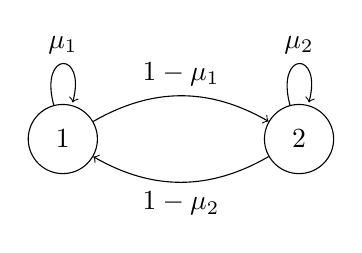
\begin{tikzpicture}[->,node distance=3cm]
    \node[state] (1)              {1};
    \node[state] (2) [right of=1] {2};

    \path (1) edge [loop above] node {$\mu_1$}   (1)
              edge [bend left,above]  node {$1-\mu_1$} (2)
          (2) edge [loop above] node {$\mu_2$}   (2)
              edge [bend left,below]  node {$1-\mu_2$} (1);
  \end{tikzpicture}
  \end{center}
  and transition matrix
  \[ P=\begin{pmatrix}\mu_1&1-\mu_1\\1-\mu_2&\mu_2\end{pmatrix} \]
  A stationary distribution $\pi$ of the transition matrix $P$ gives the proportion of times each arm is played in the long run. Let $\pi$ be a stationary distribution for $P$
  \[\begin{array}{rrcl}
    &\pi&=&\pi P\\
    \implies&(\pi_1,\ \pi_2)&=&\big(\pi_1,\ \pi_2\big)\begin{pmatrix}\mu_1&1-\mu_1\\1-\mu_2&\mu_2\end{pmatrix}\\
    \implies&(\pi_1,\ \pi_2)&=&\big(\mu_1\pi_1+\pi_2(1-\mu_2),\ \pi_1(1-\mu_1)+\pi_2\mu_2\big)\\
    \implies&\pi_1&=&\mu_1\pi_1+\pi_2(1-\mu_2)\\
    \implies&\pi_1(1-\mu_1)&=&\pi_2(1-\mu_2)\\
    \implies&\pi_1&=&\pi_2\frac{1-\mu_2}{1-\mu_1}
  \end{array}\]
  By the definition of a stationary distribution $\pi_1+\pi_2=1\implies\pi_2=1-\pi_1$. Substituting this result back in we can get explicit results for $\pi_1$ and $\pi_2$.
  \[\begin{array}{rrcl}
    &\pi_1&=&(1-\pi_1)\frac{1-\mu_2}{1-\mu_1}\\
    \implies&\pi_1\left(1+\frac{1-\mu_2}{1-\mu_1}\right)&=&\frac{1-\mu_2}{1-\mu_1}\\
    \implies&\pi_1\left(\frac{2-\mu_1-\mu_2}{1-\mu_1}\right)&=&\frac{1-\mu_2}{1-\mu_1}\\
    \implies&\pi_1&=&\frac{1-\mu_2}{2-\mu_1-\mu_2}\\
    &\pi_2&=&1-\pi_1\\
    \implies&\pi_2&=&1-\frac{1-\mu_2}{2-\mu_1-\mu_2}\\
    &&=&\frac{1-\mu_1}{2-\mu_1-\mu_2}
  \end{array}\]
  We can now create an approximate expression for the regret $\R_T$ over time horizon $T$.
  \[\begin{array}{rcl}
    \R_T&=&(\mu_1-\mu_2)\expect(\text{times arm 2 played})\\
    &=&(\mu_1-\mu_2)[T\prob(\text{arm 2 played})]\\
    &=&(\mu_1-\mu_2)T\pi_2\\
    &=&T(\mu_1-\mu_2)\frac{1-\mu_1}{2-\mu_1-\mu_2}
  \end{array}\]
\end{answer}

\begin{question}{3.}
  Consider a bandit with two independent Bernoulli arms, with mean rewards $\mu_1>\mu_2$ Define $\Delta:=\mu_1-\mu_2$. Let $N_i(t)$ denote the number of times that arm $i$ has been played in the first $t$ rounds, where $i\in\{1,2\}$ and $t\in\nats$. Let  $\hat\mu_{i,s}$ denote the empirical (or sample) mean reward obtained in the first $s$ plays of arm $i$.
  \par Suppose a genie tells you the value of $\mu_1$, the mean reward on arm 1 (but not that arm 1 is better). Then, the appropriate modification to the $UCB(\alpha)$ algorithm is as follows:
  \begin{itemize}
    \item Play arm 2 in the first round.
    \item At the end of round $t$, calculate the index of arm 2, defined answer
    \[ \iota_2(t):=\hat\mu_{2,N_2(t)}+\sqrt{\frac{\alpha\ln(t)}{2N_2(t)}} \]
    The index of arm 1 is always $\mu_1$, which is known.
    \item In round $t+1$, play the arm with the greater index, breaking ties in favour of arm 2.
  \end{itemize}
  Assume that $\alpha>1$
\end{question}

\begin{question}{3. (a)}
  Show that, if arm 2 is played by the above algorithm in round $s+1$ (i.e. $I(s+1)=2$) then one of the following statements must be true.
  \begin{enumerate}
    \item $\displaystyle N_2(s)<\frac{2\alpha\ln(s)}{\Delta^2}$
    \item $\displaystyle\hat\mu_{2,N_2(s)}\geq\mu_2+\sqrt{\frac{\alpha\ln(s)}{2N_2(s)}}$
  \end{enumerate}
\end{question}

\begin{answer}{3. (a)}
  \textit{This is a proof by contradiction}.
  \par Suppose $I(s+1)=2$ but that none of the statements above hold. Then
  \[\begin{array}{rrclcl}
    &\hat\mu_{2,N_2(s)}-\sqrt{\frac{\alpha\ln(s)}{2N_2(s)}}&<&\mu_2&\quad&\text{by not ii)}\\
    &&=&\mu_1-\Delta&&\text{by def. of }\Delta\\
    &&\leq&\mu_1-\sqrt{\frac{2\alpha\ln(s)}{N_2(s)}}&&\text{by not i)}\\
    \implies&\hat\mu_{2,N_2(s)}+\sqrt{\frac{2\alpha\ln(s)}{N_2(s)}}-\sqrt{\frac{\alpha\ln(s)}{2N_2(s)}}&<&\mu_1\\
    \implies&\hat\mu_{2,N_2(s)}+\left(\sqrt2-\frac1{\sqrt2}\right)\sqrt{\frac{\alpha\ln(s)}{N_2(s)}}&<&\mu_1\\
    \implies&\hat\mu_{2,N_2(s)}+\sqrt{\frac{\alpha\ln(s)}{2N_2(s)}}&<&\mu_1\\
    \implies&i_2(s)&<&\mu_1
  \end{array}\]
  This means $I(s+1)=1$, which is a contradiction. Thus at least one of i) or ii) must be true.
\end{answer}

\begin{question}{3. (b)}
  Recall that $N_2(t)=\sum_{s=1}^t\indexed\{I(S)=2\}$. For an arbitrary positive integer $u$ and any $t\in\nats$ explain why
  \[ N_2(t)\leq u+\sum_{s=u+1}^t\indexed\big\{\{N_2(s-1)\geq u\}\text{ and }\{I(s)=2\}\big\} \]
\end{question}

\begin{answer}{3. (b)}
  Fix $t,u\in\nats$. We have two possibilities
  \begin{itemize}
    \item[\textit{Case 1}] $N_2(t)\leq u$ (i.e. Arm two has not been played $u$ times yet). The result trivially holds in this case.
    \item[\textit{Case 2}] $\exists\ s\in[1,t]$ such that $N(s)>u$ (i.e. Arm two has been played at least $u$ times).\\ Let $s^*$ denote the smallest such $s$. Then it must be true that $N(s^*-1)=u$ and $s^*\geq u+1$. Hence
    \[\begin{array}{rclcl}
      N(t)&=&\sum_{s=1}^{s^*-1}I(s)+\sum_{s=s^*}^tI(s)&\quad&\\
      &=&N(s^*-1)+\sum_{s=s^*}^tI(s)\underbrace{\indexed\{N(s-1)\geq u\}}_\text{true for all in sum}\\
      &\leq&u+\sum_{s=u+1}^t\indexed\{N(s-1)\geq u\}&&\text{ since }s^*\geq u+1
    \end{array}\]
  \end{itemize}
  Thus the result holds in all cases.$\hfill$
\end{answer}

\begin{question}{3. (c)}
  Define $u=\left\lceil(2\alpha\ln(t))/\Delta^2\right\rceil$. Using the answers to parts \texttt{(a)} and \texttt{(b)}, and relevant probability inequalities, show that
  \[ \expect[N_2(t)\leq u+\sum_{s=u+1}^te^{-\alpha\ln(s)} \]
  Use this to show that $\expect[N_2(t)]\leq u+\frac1{\alpha-1}$.
\end{question}

\begin{answer}{3. (c)}
  We have
  \[ \expect[N_2(t)]\leq u+\sum_{s=u+1}^te^{-\alpha\ln(s)} \]
  Taking expectations of both sides
  \[\begin{array}{rcl}
  \expect[N_2(t)]&\leq&u+\sum_{s=u+1}^t\prob\left(\{N_2(s-1)\geq u\}\text{ and }\{I(s)=2\}\right)\\
  &\leq&u+\sum_{s=u}^{t-1}\prob\left(\{N_2(s)\geq u\}\text{ and }\{I(s+1)=2\}\right)
  \end{array}\]
  If $N_2(s)\geq u$ and $I(s+1)=2$ then
  \[ \hat\mu_{2,N_2(s)}\geq\mu_2+\sqrt{\frac{\alpha\ln(s)}{2N_2(s)}}\text{ by a)} \]
  Thus
  \[ \expect(N_2(t))\leq u+\sum_{s=u}^{t-1}\prob\left(\hat\mu_{2,N_2(s)}\geq\mu_2+\sqrt{\frac{\alpha\ln(s)}{2N_2(s)}}\right)\quad(1) \]
  Let $X_1,\dots,X_{N_2}$ be the random variables for each time arm 2 was played. Consider
  \[\begin{array}{rrclcl}
  &\prob\left(\hat\mu_{2,N_2(s)}\geq\mu_2+\sqrt{\frac{\alpha\ln(s)}{2N_2(s)}}\right)&=&\prob\left(\frac{1}{N_2}\sum_{i=1}^{N_2}X_i\geq\mu_2+\sqrt{\frac{\alpha\ln(s)}{2N_2(s)}}\right)&\quad&\\
  &&=&\prob\left(\sum_{i=1}^{N_2}(X_i-\mu_2)\geq N_2\sqrt{\frac{\alpha\ln(s)}{2N_2(s)}}\right)\\
  &&\leq&\text{exp}\left(-2\cdot N_2\cdot\frac{\alpha\ln(s)}{2N_2(s)}\right)&&\text{by Hoeffding's Ineq.}\\
  &&=&\text{exp}(-\alpha\ln(s))\\
  \implies&\expect[N_2(t)]&\leq&u+\sum_{s=u+1}^te^{-\alpha\ln(s)}&&\text{by (1)}
  \end{array}\]
  Further
  \[\begin{array}{rcl}
    \expect[N_2(t)]&\leq&u+\sum_{s=u+1}^te^{-\alpha\ln(s)}\\
    &=&u+\sum_{s=u+1}^ts^{-\alpha}\\
    &\leq&u+\int_u^\infty s^{-\alpha}ds\quad\text{since }\alpha>1\\
    &=&u+\left[\frac{s^{-\alpha+1}}{-\alpha+1}\right]_u^\infty\\
    &=&u-\frac{u^{-\alpha+1}}{-\alpha+1}\\
    &=&u+\frac{u^{-\alpha+1}}{\alpha+1}
  \end{array}\]
  By the definition of $u$, $u>1$ thus $u^{-\alpha+1}<1$ since $\alpha>1$. Giving us
  \[ \expect[N_2(t)]\leq u+\frac1{\alpha-1} \]
\end{answer}

\begin{question}{3. (d)}
  Use the answer to \texttt{(c)} to show that the regret of this algorithm is bounded above as
  \[ \mathcal{R}(T)\leq\frac{2\alpha\ln(T)}\Delta+\frac{\alpha}{\alpha-1}\Delta \]
\end{question}

\begin{answer}{3. (d)}
  \[\begin{array}{rrlcl}
  \mathcal{R}(T)&:=&\Delta\expect[N_2(t)]&\quad&\\
  &\leq&\Delta\left(u+\frac1{\alpha-1}\right)&&\text{by 3. (c)}\\
  &\leq&\Delta\left(\frac{2\alpha\ln(T)}{\Delta^2}+1+\frac1{\alpha-1}\right)&&\text{by def. of }u\\
  &=&\frac{2\alpha\ln(T)}{\Delta}+\Delta\left(1+\frac1{\alpha-1}\right)\\
  &=&\frac{2\alpha\ln(T)}{\Delta}+\frac{\Delta\alpha}{\alpha-1}
  \end{array}\]
\end{answer}

\begin{question}{4.}
  Consider a bandit with two independent Gaussian arms. Rewards on arm $i$ constitute a sequence of iid $N(\mu_i,1)$ random variables.
\end{question}

\begin{question}{4. (a)}
  Let $\hat\mu_{i,n}$ denote the sample mean reward on arm $i$ after $n$ plays of this arms. Using a resulting from Homework 1, show that
  \[ \prob\left(\hat\mu_{i,n}<\mu_i+\sqrt{\frac{\alpha\ln(t}{2n}}\right)\leq\exp\left(-\frac{\alpha\ln(t)}4\right) \]
  Express the last quantity as power of $t$.
\end{question}

\begin{answer}{4. (a)}
  Let $\hat\mu_{i,n}$ be the sample mean reward on arm $i$ after $n$ plays of that arms.
  \par From \textit{Problem Sheet 1 6b)}, for $X_i\iid\text{Normal}(\mu,\sigma^2)$ and $\gamma>\mu_i$ we have that
  \[ \prob(\hat\mu>\gamma)=\prob\left(\sum_{i=1}^n X_i>n\gamma\right)\leq\exp\left(-n\frac{(\gamma-\mu)^2}{2\sigma^2}\right) \]
  Applying this result to this scenario
  \[ \prob(\hat\mu_{i,n}>\gamma)\leq\exp\left(-n\frac{(\gamma-\mu_i)^2}2\right) \]
  By defining $\gamma=\mu_i+\sqrt{\frac{\alpha\ln(t)}{2n}}$ with $\alpha>0$.
  \par Note that $\gamma>\mu_i$ so we can use the above inequality
  \[\begin{array}{rcl}
  \prob\left(\hat\mu_{i,n}>\mu_i+\sqrt{\frac{\alpha\ln(t)}{2n}}\right)&\leq&\exp\left(-\frac{n}2\cdot\frac{\alpha\ln(t)}{2n}\right)\\
  &=&\exp\left(-\frac{\alpha\ln(t)}4\right)\\
  &=&t^{-\alpha/4}
  \end{array}\]
\end{answer}

\begin{question}{4. (b)}
  Explain in a few sentences why the same bound holds the probability of the event that $\hat\mu_{i,n}<\mu_i-\sqrt{\frac{\alpha\ln(t)}{2n}}$
\end{question}

\begin{answer}{4. (b)}
  The result from \textit{Problem Sheet 1 6b)} is derived from the Chernoff Bound for IID random variables when $\left\{\sum X_i\geq nc\right\}$ and considers $\inf_{\theta>0}e^{-n\theta c}(\expect[e^{\theta X}])^n$. The result requires $c>\mu_i$ in order to fulfil the restriction on the infimum (i.e. $\theta>0$).
  \par To derive a similar result to \textit{Question 4. (a)} for the event $\textstyle\left\{\hat\mu_{i,n}<\mu_i-\sqrt{\frac{\alpha\ln(t)}{2n}}\right\}$ we define $c=\mu_i-\sqrt{\frac{\alpha\ln(t)}{2n}}$, meaning $c<\mu_i$ and thus $\theta<0$, for the $\theta$ in the infimum.
  \par The Chernoff Bound for this complementary event considers the infimum of the same expression, except with the restriction that $\theta<0$ (rather than $\theta>0$). Given our definition of $c$ and the resulting value of $\theta$, the same value for the infimum is found. Meaning the same bound is derived for both the event and its compliment.
\end{answer}

\begin{question}{4. (c)}
  Replicate the analysis of the UCB algorithm to obtain a regret bound of the form $\mathcal{R}(T)\leq c_1+c_2\ln(T)$ where $c_1$ and $c_2$ are constants that may depend on $\alpha,\mu_1$ and $\mu_2$. Find explicit expressions for these constants.
  \par The analysis will not work for all $\alpha>1$. You will need $\alpha$ to be bigger than some other number. Find that number.
\end{question}

\begin{answer}{4. (c)}
  Assume WLOG $\mu_1>\mu_2$ and define $\Delta=\mu_1-\mu_2$. Let $N_2(t)$ be the number of times arm 2 is played in the first $t$ steps. Define $u_t=\left\lceil\frac{2\alpha\ln(t)}{\Delta^2}\right\rceil$. We have
  \[ N_2(t)\leq u+\sum_{s=u-1}^t\indexed\left(\left\{N_2(s-1)\geq u_t\right\}\text{ and }\{I(s)=j\}\right) \]
  Taking expectations of both side we get
  \[ \expect[N_2(t)]\leq u_t+\sum_{s=u_t}^{t-1}\prob\left(\{N_2(s-1)\geq u_t\}\text{ and }\{I(s)=j\}\right) \]
  By considering the two cases where the sub-optimal arm is played: $\hat\mu_1$ is significantly lower than $\mu_1$; or $\hat\mu_2$ is significantly higher than $\mu_2$.
  \[\begin{array}{rcl}
    \expect[N_2(t)]&\leq&u_t+\sum_{s=u_t}^{t-1}\left[\prob\left(\hat\mu_{1,N_1(s)}\leq\mu_1-\sqrt{\frac{\alpha\ln(s)}{2N_2(s)}}\right)+\prob\left(\hat\mu_{2,N_2(s)}>\mu_2-\sqrt{\frac{\alpha\ln(s)}{2N_2(s)}}\right)\right]\\
    &\leq&u_t+\sum_{s=u_t}^{t-1}2t^{-\alpha/4}\text{ by \textit{Question 4. (a)}}\\
    &\leq&u+\int_{u_t-1}^\infty2t^{-\alpha/4}dt\\
    &=&u_t+2\left[\frac{t^{-\frac\alpha4+1}}{1-\frac\alpha4}\right]\limits_{u_t-1}^\infty\\
    &=&u_t-\frac{2(u_t-1)^{-\frac\alpha4+1}}{-\frac{\alpha}4+1}\\
    &\leq&u_t+\frac{2}{\frac\alpha4-1}\\
    &=&u_t+\frac8{\alpha-4}\\
    &\leq&\frac{2\alpha\ln(t)}{\Delta^2}+1+\frac8{\alpha-4}\text{ by def. of }u_t\\
    &=&\frac{2\alpha\ln(t)}{\Delta^2}+\frac{\alpha+4}{\alpha-4}
  \end{array}\]
  In this scenario $\mathcal{R}(T)=\Delta\expect[N_2(T)]$. Thus, using the results above
  \[ \mathcal{R}(T)\leq\frac{2\alpha\ln(T)}{\Delta}+\Delta\frac{\alpha+4}{\alpha-4} \]
  This requires $\alpha>4$.
\end{answer}

\begin{question}{5.}
  Let $X\sim\text{Bern}(p)$ and $Y\sim\text{Bern}(q)$ with $p,q\in[0,1]$. Recall that the KL-Divergence of a $\text{Bern}(q)$ distribution wrt a $\text{Bern}(p)$ distribution is defined as
  \[ KL(q;p):=q\ln\left(\frac{q}p\right)+(1-q)\ln\left(\frac{1-q}{1-p}\right) \]
  with $x\ln(x)$ defined to be zero if $x$ is zero. Recall also that the total variation distance between these distributions, denoted $d_{TV}(\text{Bern}(q),\text{Bern}(p)):=|q-p|$. Prove \textit{Pinsker's Inequality} which states
  \[ KL(q;p)\geq2\big(\text{Bern}(q),\text{Bern}(p)\big)^2\]
\end{question}

\begin{answer}{5.}
  Fix the value of $p$ and define the consider the following function
  \[\begin{array}{rrl}
    f(q)&:=&KL(q;p)-2(q-p)^2\\
    &=&q\ln\left(\frac{q}p\right)+(1-q)\ln\left(\frac{1-q}{1-p}\right)-2(q-p)^2\text{ by def of }KL
  \end{array}\]
  I will show that this function is convex
  \[\begin{array}{rcl}
    f'(q)&=&\ln\left(\frac{q}p\right)+q\cdot\frac{1/p}{q/p}-\ln\left(\frac{1-q}{1-p}\right)+(1-q)\frac{-1/(1-p)}{(1-q)/(1-p)}-4(q-p)\\
    &=&\ln\left(\frac{q}p\right)-\ln\left(\frac{1-q}{1-p}\right)-4(q-p)\\
    f''(q)&=&\frac{1/p}{q/p}-\frac{-1/(1-p)}{(1-q)/(1-p)}-4\\
    &=&\frac1q+\frac1{1-q}-4\\
    &=&\frac1{q(1-q)}-4
  \end{array}\]
  Note $\underset{q\in(0,1)}\min\frac1{q(1-q)}=\frac1{\frac12(1-\frac12)}=4$. Thus $\frac1{q(1-q)}\geq 4\ \forall\ q\in(0,1)$.
  Further, $f''(q)\geq0$ for the whole domain $q\in(0,1)$, meaning $f(q)$ is convex.
  \par Now note that $f'(p)=0$ (ie the minimum occurs when $q=p$) and that $f(p)=0$ (ie $\underset{q\in(0,1)}\min f(q)=0$), this means $f(q)\geq f(p)=0\ \forall\ q\in(0,1)$.
  \par Using this inequality we can finally derive \textit{Pinsker's Inequality} for Bernoulli random variables
  \[\begin{array}{rrcl}
    &f(q)&\geq&0\\
    \implies&K(q;p)-2(q-p)^2&\geq&0\\
    \implies&K(q;p)&\geq&2(q-p)^2=2|q-p|^2\\
    &&=&2d_{TV}(\text{Bern}(q),\text{Bern}(p))^2
  \end{array}\]
  This is \textit{Pinsker's Inequality} for Bernoulli random variables.
\end{answer}

% \begin{question}{6.}
%   Let $X$ and $Y$ be random variables with probability distributions $P$ and $Q$ respectively. Suppose $P$ and $Q$ have densities $p$ and $q$ wrt a reference measure $m$ (Usually $m$ is Lebesgue measure on the real line). Then the KL-Divergence of $Q$ wrt $P$ is defined as
%   \[ KL(Q;P):=\int q(x)\ln\left(\frac{q(x)}{p(x)}\right)dm(x) \]
%   (If $M $ is the Lebesgue measure, we just write $dx$ instead of $dm(x)$).
%   \par In the following you may use, without proof, the fact which follows from Jensen's inequality
%   \[ KL(Q,P)\geq 0\quad\forall\ Q,P \]
%   The total variation distance between $P$ and $Q$ (which is symmetric) is defined as
%   \[ d_{TV}(Q,P):=\sup_A|Q(A)-P(A)| \]
%   where $P(A)$ and $Q(A)$ are the probabilities of the event set $A$ under the probability measure $P$ and $Q$. The supremum is taken over all measure sets $A$
% \end{question}
%
% \begin{question}{6. (a)}
%   Let $A^*:=\{x:q(x)\geq p(x)\}$. Explain why $d_{TV}(Q,P)=Q(A^*)-P(A^*)$. Maybe use a Venn diagram (a formal prove is not required).
% \end{question}
%
% \begin{answer}{6. (a)}
%   TODO
% \end{answer}
%
% \begin{question}{6. (b)}
%   For any measureable set $A$ such that $P(A)$ is not equal to zero \underline{or} one. Show that
%   \[ KL(Q,P)\geq K(Q(A),P(A)) \]
%   where the term on the right refers to the KL-Divergence of a $\text{Bern}(Q(A))$ distribution wrt a $\text{Bern}(P(A))$ distribution.
%
% \end{question}
%
% \begin{answer}{6. (b)}
%   TODO
% \end{answer}
%
% \begin{question}{6. (c)}
%   Using the answers from the last two parts, prove the general version of Pinsker's inequality, which states that for any two probability measures $P$ and $Q$ (ie not just Bernoulli)
%   \[ KL(Q;P)\geq 2(d_{TV}(Q,P))^2 \]
% \end{question}
%
% \begin{answer}{6. (c)}
%   TODO
% \end{answer}

\end{document}
